\documentclass[12pt,a4paper]{article}

% ─── Page Layout ───────────────────────────────────────────────────────────────
\usepackage[a4paper, margin=0.8in, headheight=14pt]{geometry}

% ─── Fonts (XeLaTeX) ───────────────────────────────────────────────────────────
\usepackage{fontspec}
\usepackage{unicode-math}
\setmainfont{TeX Gyre Pagella}
\setmonofont[Scale=0.88]{TeX Gyre Cursor}
\setmathfont{Latin Modern Math}

% ─── Packages ──────────────────────────────────────────────────────────────────
\usepackage{xcolor}
\usepackage{colortbl}
\usepackage{titlesec}
\usepackage{enumitem}
\usepackage{tabularx}
\usepackage{booktabs}
\usepackage{array}
\usepackage{amsmath}
\usepackage{tikz}
\usetikzlibrary{shapes.geometric, arrows.meta, positioning, calc, fit, decorations.pathreplacing}
\usepackage{tcolorbox}
\tcbuselibrary{skins, breakable}
\usepackage{hyperref}
\usepackage{fancyhdr}
\usepackage{graphicx}
\usepackage{microtype}
\hyphenpenalty=10000
\exhyphenpenalty=10000
\sloppy
\usepackage{caption}
\usepackage{setspace}
\usepackage{multirow}
\usepackage{tocloft}

% ─── Q&A helper ────────────────────────────────────────────────────────────────
\newcommand{\Q}[1]{\textbf{#1}\par\noindent\ignorespaces}

% ─── Colour Palette ────────────────────────────────────────────────────────────
\definecolor{myred}{RGB}{196,30,58}
\definecolor{mydark}{RGB}{30,30,50}
\definecolor{mygreen}{RGB}{14,120,80}
\definecolor{myteal}{RGB}{0,130,140}
\definecolor{myamber}{RGB}{180,100,0}
\definecolor{mypurple}{RGB}{100,30,160}
\definecolor{mygray}{RGB}{246,247,249}
\definecolor{mgframe}{RGB}{180,185,200}
\definecolor{watermark}{RGB}{145,150,170}
\definecolor{hdrred}{RGB}{250,232,235}
\definecolor{hdrgreen}{RGB}{220,244,233}
\definecolor{hdrteal}{RGB}{220,242,244}
\definecolor{hdramber}{RGB}{253,242,215}
\definecolor{hdrpurple}{RGB}{238,228,255}
\definecolor{hdrgray}{RGB}{238,240,245}
\definecolor{rowalt}{RGB}{250,251,253}

% ─── Section Formatting ────────────────────────────────────────────────────────
\titleformat{\section}
  {\large\bfseries\color{myred}}{\thesection.}{0.5em}{}
  [\vspace{1pt}{\color{myred}\rule{\linewidth}{0.8pt}}]
\titleformat{\subsection}
  {\normalsize\bfseries\color{myteal}}{\thesubsection}{0.5em}{}
\titlespacing*{\section}{0pt}{18pt}{7pt}
\titlespacing*{\subsection}{0pt}{11pt}{4pt}

% ─── Paragraph ─────────────────────────────────────────────────────────────────
\setlength{\parindent}{0pt}
\setlength{\parskip}{4pt}

% ─── TOC Styling ───────────────────────────────────────────────────────────────
\renewcommand{\cfttoctitlefont}{\large\bfseries\color{myred}}
\renewcommand{\cftaftertoctitle}{\par\noindent{\color{myred}\rule{\linewidth}{0.8pt}}}
\setlength{\cftbeforetoctitleskip}{0pt}
\setlength{\cftaftertoctitleskip}{6pt}
\renewcommand{\cftsecfont}{\normalsize\bfseries\color{mydark}}
\renewcommand{\cftsecpagefont}{\normalsize\bfseries\color{mydark}}
\renewcommand{\cftsecleader}{\cftdotfill{\cftdotsep}}
\setlength{\cftbeforesecskip}{7pt}
\renewcommand{\cftsubsecfont}{\small\color{mydark}}
\renewcommand{\cftsubsecpagefont}{\small\color{mydark}}
\setlength{\cftbeforesubsecskip}{3pt}
\setlength{\cftsubsecindent}{1.4em}

% ─── Table helpers ─────────────────────────────────────────────────────────────
\renewcommand{\arraystretch}{1.45}
\setlength{\tabcolsep}{6pt}
\arrayrulecolor{mydark}
\newcolumntype{B}[1]{>{\small\bfseries\raggedright\arraybackslash}m{#1}}
\newcolumntype{Y}{>{\small\raggedright\arraybackslash}X}
\renewcommand{\tabularxcolumn}[1]{m{#1}}

% ─── Header / Footer ───────────────────────────────────────────────────────────
\pagestyle{fancy}
\fancyhf{}
\fancyhead[L]{\small\color{myred}\textbf{PE-EC701B}\;\color{mydark}--- Satellite Communication}
\fancyhead[R]{\small\color{myteal}\textbf{Module 6 Notes}}
\fancyfoot[C]{\small\color{mydark}\thepage}
\fancyfoot[R]{\small\color{watermark}\textit{\copyright\ Biraj}}
\renewcommand{\headrulewidth}{0.5pt}
\renewcommand{\footrulewidth}{0.3pt}

% ─── Hyperref ──────────────────────────────────────────────────────────────────
\hypersetup{
  colorlinks=true, linkcolor=myteal, urlcolor=myteal,
  pdfauthor={Biraj Sarkar},
  pdftitle={PE-EC701B --- Module 6 Notes}
}

% ─── tcolorbox styles ──────────────────────────────────────────────────────────
\tcbset{
  tikzbox/.style={
    colback=mygray, colframe=mgframe, boxrule=0.6pt, arc=4pt,
    left=8pt, right=8pt, top=6pt, bottom=6pt,
    colbacktitle=mgframe, coltitle=mydark,
    fonttitle=\small\bfseries
  },
  defbox/.style={
    colback=hdrgreen, colframe=mygreen, boxrule=0.8pt, arc=4pt,
    left=9pt, right=9pt, top=6pt, bottom=6pt,
    colbacktitle=mygreen, coltitle=white,
    fonttitle=\small\bfseries
  },
  formulabox/.style={
    colback=hdrteal, colframe=myteal, boxrule=0.8pt, arc=4pt,
    left=9pt, right=9pt, top=7pt, bottom=7pt,
    colbacktitle=myteal, coltitle=white,
    fonttitle=\small\bfseries
  },
  examplebox/.style={
    colback=hdramber, colframe=myamber, boxrule=0.8pt, arc=4pt,
    left=9pt, right=9pt, top=6pt, bottom=6pt,
    colbacktitle=myamber, coltitle=white,
    fonttitle=\small\bfseries
  },
  masonbox/.style={
    colback=hdrpurple, colframe=mypurple, boxrule=0.8pt, arc=4pt,
    left=9pt, right=9pt, top=6pt, bottom=6pt,
    colbacktitle=mypurple, coltitle=white,
    fonttitle=\small\bfseries
  },
  exambox/.style={
    colback=hdrpurple, colframe=mypurple, boxrule=1pt, arc=5pt,
    left=10pt, right=10pt, top=8pt, bottom=8pt,
    colbacktitle=mypurple, coltitle=white,
    fonttitle=\bfseries,
    breakable, title after break={\textbf{Frequently Asked / Viva Questions (contd.)}}}
}
% Make all boxes breakable across pages
\tcbset{breakable}

% ─── TikZ styles ───────────────────────────────────────────────────────────────
\tikzset{
  block/.style={rectangle, draw=myteal, fill=hdrteal,
    text width=2.4cm, align=center, minimum height=0.95cm,
    font=\small, rounded corners=3pt, line width=0.7pt},
  redblock/.style={rectangle, draw=myred, fill=hdrred,
    text width=2.4cm, align=center, minimum height=0.95cm,
    font=\small, rounded corners=3pt, line width=0.7pt},
  netnode/.style={rectangle, draw=myteal, fill=hdrteal,
    text width=1.5cm, align=center, minimum height=0.8cm,
    font=\small, rounded corners=3pt, line width=0.7pt},
  sumjunc/.style={circle, draw=myamber, fill=hdramber,
    minimum size=0.62cm, font=\small, line width=0.8pt},
  snode/.style={circle, draw=mypurple, fill=hdrpurple,
    minimum size=0.55cm, font=\footnotesize, line width=0.7pt},
  arrow/.style={-Stealth, thick, color=mydark},
  redarrow/.style={-Stealth, thick, color=myred},
  line/.style={thick, color=mydark}
}

% ═══════════════════════════════════════════════════════════════════════════════
\begin{document}
% ═══════════════════════════════════════════════════════════════════════════════

\begin{center}
  {\LARGE\bfseries\color{myred} PE-EC701B --- Satellite Communication}\\[5pt]
  {\normalsize\color{mydark} Semester VII \quad$\bullet$\quad 3L:0T:0P \quad$\bullet$\quad 3 Credits}\\[3pt]
  {\normalsize\color{myteal}\textbf{Module 6 Exam Notes: Modulation and Multiple Access Schemes}}\\[3pt]
  {\small\color{mydark} CGEC \;$|$\; B.Tech ECE (2023--27) \;$|$\; \textit{Biraj Sarkar}}
\end{center}
\vspace{2pt}
\noindent{\color{myred}\rule{\linewidth}{1.5pt}}
\vspace{2pt}

\hypersetup{linkcolor=mydark}
\tableofcontents
\hypersetup{linkcolor=myteal}
\newpage

% ===============================================================================
\section{Modulation Schemes in Satellite Communication}
% ===============================================================================

Modulation is the process of mapping digital baseband information onto a high-frequency analog carrier wave suitable for transmission through space.

\begin{tcolorbox}[defbox]
\textbf{Digital Modulation in Satcom:} The translation of binary sequences into discrete phase or amplitude shifts of a microwave carrier. Because satellite transponders are power-limited, phase-shift keying (PSK) schemes like QPSK are preferred over amplitude-modulated schemes.
\end{tcolorbox}

\subsection{Why QPSK is the Industry Workhorse}
\begin{itemize}[leftmargin=*, itemsep=3.5pt]
  \item \textbf{Constant Envelope:} QPSK has a constant envelope (its amplitude does not vary with phase shifts). This allows the satellite high-power amplifier (HPA) to operate at its maximum efficiency point (saturation) without introducing severe \textbf{amplitude-to-phase distortion (AM/PM)}.
  \item \textbf{Spectral Efficiency:} QPSK offers double the spectral efficiency of BPSK ($2 \text{ bps/Hz}$ vs. $1 \text{ bps/Hz}$) for the same noise performance.
  \item \textbf{Higher-Order Modulation:} Systems requiring higher data rates (such as DTH satellite TV) use \textbf{8PSK} or \textbf{16APSK} (Amplitude Phase Shift Keying) coupled with advanced forward error correction (FEC) under the DVB-S2 standard.
\end{itemize}

% ===============================================================================
\section{Concept of Multiple Access}
% ===============================================================================

A communication satellite serves as a central hub. \textbf{Multiple Access} is the set of traffic-sharing protocols that allow multiple geographically separated ground terminals to transmit signals simultaneously through a single satellite transponder.

\begin{tcolorbox}[defbox]
\textbf{Multiple Access:} The technique of sharing a common channel resource (transponder bandwidth and power) among multiple users without causing mutual electromagnetic interference.
\end{tcolorbox}

\subsection{Sharing Methodologies}
The three primary sharing mechanisms are:
\begin{enumerate}[label=\textbf{\arabic*.}, leftmargin=*, itemsep=2.5pt]
  \item \textbf{FDMA:} Resource split by Frequency.
  \item \textbf{TDMA:} Resource split by Time.
  \item \textbf{CDMA:} Resource split by mathematical Codes.
\end{enumerate}

\begin{tcolorbox}[tikzbox, title={Multiple Access Resource Partitioning}]
\centering
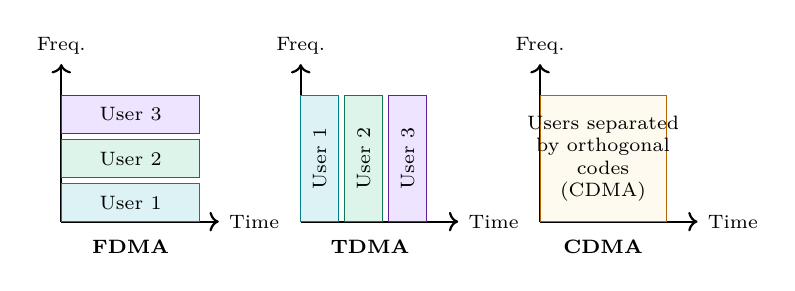
\begin{tikzpicture}[scale=0.8, every node/.style={font=\scriptsize}]
  % FDMA Grid
  \begin{scope}[xshift=0cm]
    \draw[thick, ->] (0,0) -- (2.5,0) node[right] {Time};
    \draw[thick, ->] (0,0) -- (0,2.5) node[above] {Freq.};
    \draw[fill=hdrteal, draw=myteal] (0,0) rectangle (2.2,0.6);
    \draw[fill=hdrgreen, draw=mygreen] (0,0.7) rectangle (2.2,1.3);
    \draw[fill=hdrpurple, draw=mypurple] (0,1.4) rectangle (2.2,2.0);
    \node at (1.1,0.3) {User 1};
    \node at (1.1,1.0) {User 2};
    \node at (1.1,1.7) {User 3};
    \node at (1.1,-0.4) {\textbf{FDMA}};
  \end{scope}
  
  % TDMA Grid
  \begin{scope}[xshift=3.8cm]
    \draw[thick, ->] (0,0) -- (2.5,0) node[right] {Time};
    \draw[thick, ->] (0,0) -- (0,2.5) node[above] {Freq.};
    \draw[fill=hdrteal, draw=myteal] (0,0) rectangle (0.6,2.0);
    \draw[fill=hdrgreen, draw=mygreen] (0.7,0) rectangle (1.3,2.0);
    \draw[fill=hdrpurple, draw=mypurple] (1.4,0) rectangle (2.0,2.0);
    \node[rotate=90] at (0.3,1.0) {User 1};
    \node[rotate=90] at (1.0,1.0) {User 2};
    \node[rotate=90] at (1.7,1.0) {User 3};
    \node at (1.1,-0.4) {\textbf{TDMA}};
  \end{scope}
  
  % CDMA Grid
  \begin{scope}[xshift=7.6cm]
    \draw[thick, ->] (0,0) -- (2.5,0) node[right] {Time};
    \draw[thick, ->] (0,0) -- (0,2.5) node[above] {Freq.};
    \draw[fill=hdramber!40, draw=myamber] (0,0) rectangle (2.0,2.0);
    \node[align=center] at (1.0,1.0) {Users separated\\by orthogonal\\codes\\(CDMA)};
    \node at (1.0,-0.4) {\textbf{CDMA}};
  \end{scope}
\end{tikzpicture}
\tcbset{colbacktitle=myteal, coltitle=white}
\end{tcolorbox}

% ===============================================================================
\section{Frequency Division Multiple Access (FDMA)}
% ===============================================================================

In FDMA, the transponder bandwidth is divided into smaller, non-overlapping frequency channels. Each Earth station is assigned a dedicated carrier frequency and transmits continuously.

\subsection{FDM vs. FDMA}
\begin{itemize}[leftmargin=*, itemsep=3.5pt]
  \item \textbf{FDM (Frequency Division Multiplexing):} A terrestrial process where multiple analog signals are combined at a single transmitter into a single composite signal.
  \item \textbf{FDMA (Multiple Access):} An uplink sharing process where multiple physically separate ground transmitters send distinct carriers to the satellite.
\end{itemize}

\subsection{Intermodulation Noise and Back-Off}
When multiple carrier waves pass through the satellite's high-power amplifier (HPA), the HPA's non-linear characteristics mix the carriers, generating \textbf{intermodulation distortion (IMD)} products.
To minimize IMD, the amplifier must be operated in its linear region rather than at saturation. This requires \textbf{Amplifier Back-Off}:
\begin{itemize}[leftmargin=*, itemsep=3.5pt]
  \item \textbf{Input Back-Off (IBO):} Reducing the input signal power below the level that drives the HPA to saturation.
  \item \textbf{Output Back-Off (OBO):} The resulting reduction in output transmit power (typically 3 to 6 dB), which reduces transponder efficiency.
\end{itemize}

% ===============================================================================
\section{Time Division Multiple Access (TDMA)}
% ===============================================================================

In TDMA, the entire transponder bandwidth is allocated to one Earth station at a time. Each station transmits data in high-speed, non-overlapping periodic bursts.

\subsection{TDMA Frame Structure}
The transmissions are organized into periodic TDMA frames. A frame consists of a preamble and traffic bursts.

\begin{itemize}[leftmargin=*, itemsep=3.5pt]
  \item \textbf{Preamble:} Contains carrier synchronization bits and unique words for time alignment.
  \item \textbf{Guard Times ($t_g$):} Small silent intervals left between adjacent bursts to prevent overlap caused by propagation delay variations.
\end{itemize}

\subsection{Frame Efficiency (\texorpdfstring{$\eta_f$}{eta\_f})}
Because guard times and preambles carry no user information, they represent overhead. The frame efficiency ($\eta_f$) is:
\begin{equation}
  \eta_f = 1 - \frac{T_{overhead}}{T_f} = 1 - \frac{N \cdot t_{preamble} + N \cdot t_g}{T_f}
\end{equation}
Where:
\begin{itemize}[leftmargin=*, itemsep=3pt]
  \item $T_f$ = Total frame duration
  \item $N$ = Number of traffic bursts (users) in the frame
  \item $t_{preamble}$ = Duration of the preamble sequence
  \item $t_g$ = Guard time duration
\end{itemize}

% ===============================================================================
\section{Code Division Multiple Access (CDMA)}
% ===============================================================================

In CDMA, all Earth stations transmit simultaneously over the entire transponder bandwidth. Users are separated using unique, orthogonal pseudo-noise (PN) codes.

\subsection{Direct Sequence Spread Spectrum (DS-CDMA)}
The baseband binary data stream is multiplied by a high-rate PN code (chipping sequence). This spreads the signal bandwidth over the entire transponder band. At the receiver, the signal is multiplied by the identical synchronized PN code to collapse the signal back to its original bandwidth (de-spreading), while all other users' signals remain spread as low-power background noise.

\subsection{Processing Gain ($G_p$)}
The ratio of the spread bandwidth ($B_{ss}$) to the baseband data bandwidth ($B_{data}$) determines the processing gain:
\begin{equation}
  G_p = \frac{B_{ss}}{B_{data}} \approx \frac{R_c}{R_d}
\end{equation}
Where $R_c$ is the chip rate (chips/sec) and $R_d$ is the baseband data rate (bits/sec).
In decibels:
\begin{equation}
  G_{p\_dB} = 10 \log_{10}\left( \frac{R_c}{R_d} \right)
\end{equation}
A higher processing gain provides greater immunity to interference and jamming.

% ===============================================================================
% MANDATORY QUICK REVISION PAGE
% ===============================================================================
\newpage
\begin{center}
  {\large\bfseries\color{myred} Quick Revision --- Module VI}\\[3pt]
  {\small\color{mydark} Modulation and Multiple Access Schemes $|$ PE-EC701B}
\end{center}
\noindent{\color{myred}\rule{\linewidth}{1.2pt}}
\vspace{4pt}

\begin{tcolorbox}[formulabox, title={\textbf{Key Formulas at a Glance}}]
\renewcommand{\arraystretch}{1.9}
\begin{tabularx}{\linewidth}{B{5.0cm} X}
QPSK Bandwidth Efficiency & $\displaystyle \eta_{bps} = \frac{R}{B} = 2 \text{ bits/sec/Hz}$ \\[4pt]
TDMA Frame Efficiency & $\displaystyle \eta_f = 1 - \frac{N(t_{preamble} + t_g)}{T_f}$ \\[4pt]
CDMA Processing Gain & $\displaystyle G_p = \frac{B_{ss}}{B_{data}} \approx \frac{R_c}{R_d}$ \\[4pt]
IMD Product Frequencies & $f_{IMD} = 2f_1 - f_2$ \quad and \quad $2f_2 - f_1$ \quad (third-order products)
\end{tabularx}
\end{tcolorbox}

\begin{tcolorbox}[defbox, title={\textbf{One-Line Definitions}}]
\begin{itemize}[leftmargin=*, itemsep=2.5pt, topsep=0pt]
  \item \textbf{Modulation:} Imprinting low-frequency signal data onto a high-frequency carrier.
  \item \textbf{Multiple Access:} Sharing a single satellite transponder's resource among multiple ground stations.
  \item \textbf{Guard Time:} Idle time slots inserted between TDMA bursts to prevent data collisions.
  \item \textbf{Back-Off:} Operation of an HPA below its saturation point to prevent intermodulation noise.
  \item \textbf{Processing Gain:} The bandwidth ratio in CDMA indicating interference suppression capability.
  \item \textbf{PN Code:} Pseudo-Noise binary code sequence used in CDMA to spread user signals.
\end{itemize}
\end{tcolorbox}

\begin{tcolorbox}[exambox, title={\textbf{Frequently Asked / Viva Questions}}]
\begin{enumerate}[topsep=0pt, label=\textbf{Q\arabic*.}, itemsep=5pt]
  \item \Q{Why are constant-envelope modulation schemes preferred in satellite communications?}
    Because satellite power amplifiers (TWTAs) are non-linear near saturation. Constant-envelope schemes like QPSK keep the carrier amplitude fixed, preventing severe non-linear amplitude distortion (AM/PM).
  \item \Q{Explain the difference between Multiplexing and Multiple Access.}
    Multiplexing is a local process combining signals at a single physical transmitter. Multiple Access is a distributed process where multiple independent transmitters coordinate to share a remote receiver.
  \item \Q{What is intermodulation distortion (IMD) in FDMA systems?}
    When multiple carrier signals pass through a non-linear amplifier (like a satellite HPA), they mix together, generating unwanted spurious frequency products (like $2f_1 - f_2$) that fall into adjacent channels.
  \item \Q{How is IMD mitigated, and what is its operational cost?}
    It is mitigated by "amplifier back-off" (reducing input power to operate in the linear region). The cost is reduced downlink transmit power (OBO), decreasing transponder power efficiency.
  \item \Q{Explain the purpose of the Guard Time ($t_g$) in TDMA.}
    Because ground stations are at different distances from the satellite, their burst transit times differ. Guard times absorb these timing variations, preventing collisions.
  \item \Q{Define TDMA frame efficiency.}
    The ratio of usable user data time slots to the total frame time: $\eta_f = 1 - T_{overhead}/T_f$.
  \item \Q{How does CDMA separate different user signals if they share the same time and frequency?}
    Each user is assigned a unique, mathematically orthogonal pseudo-noise (PN) code. The receiver correlates the composite signal with the desired user's code, recovering the data while treating other users as thermal noise.
  \item \Q{Calculate the processing gain (in dB) of a CDMA system with a baseband data rate of 9.6 kbps and a chip rate of 1.2288 Mcps.}
    $G_p = 1.2288 \times 10^6 / 9.6 \times 10^3 = 128$. In dB: $10\log_{10}(128) \approx 21.07 \text{ dB}$.
  \item \Q{What is the difference between Direct Sequence (DS) and Frequency Hopping (FH) CDMA?}
    DS-CDMA multiplies the signal by a fast PN code continuously. FH-CDMA shifts the carrier frequency rapidly in a pseudo-random pattern.
  \item \Q{Why does TDMA require complex synchronization compared to FDMA?}
    Because TDMA relies on precise time slots. Ground stations must adjust their transmission timing within microseconds to match the satellite frame clock.
  \item \Q{What is the Near-Far effect in CDMA and how is it resolved?}
    An Earth station closer to the satellite will overwhelm the signals from farther stations. It is resolved using dynamic uplink power control (UPC) to ensure all signals arrive at the satellite with equal power.
  \item \Q{Which multiple access scheme is most suitable for bursty data traffic?}
    CDMA or TDMA with demand-assigned multiple access (DAMA), which allocates slots dynamically on demand, whereas fixed FDMA is inefficient for bursty traffic.
\end{enumerate}
\end{tcolorbox}

\begin{tcolorbox}[tikzbox, title={Comparison of FDMA, TDMA, and CDMA}]
\renewcommand{\arraystretch}{1.4}
\par\noindent
{\renewcommand{\arraystretch}{1.55}%
\begin{tabularx}{\linewidth}{|B{3.2cm}|Y|Y|Y|}
\hline
\textbf{Parameter} & \textbf{\color{myteal}FDMA} & \textbf{\color{myred}TDMA} & \textbf{\color{myamber}CDMA} \\[4pt]
\hline
\textbf{Resource Allocation} & Dedicated frequency slots, continuous transmission. & Dedicated time slots, full bandwidth bursts. & Shared time and frequency, separated by codes. \\[4pt]
\hline
\textbf{IMD Vulnerability} & High (requires back-off). & Negligible (only one carrier in transponder at a time). & Low (mitigated by code orthogonality). \\[4pt]
\hline
\textbf{Complexity} & Low; simple frequency filters at receiver. & High; requires precise time synchronization. & High; requires complex code generators and correlators. \\[4pt]
\hline
\textbf{Flexibility} & Rigid; channel bandwidth is fixed. & Flexible; slots can be dynamically reallocated. & High; soft capacity limit (adding users degrades noise floor). \\[4pt]
\hline
\end{tabularx}
}
\end{tcolorbox}

\end{document}
